\documentclass[11pt]{article}
\usepackage[a4paper, margin=2cm]{geometry}
\usepackage[utf8]{inputenc}
\usepackage{babel}
\usepackage[spanish]{layout}
\usepackage[article]{ragged2e}
\usepackage{textcomp}
\usepackage{amsmath}
\usepackage{amssymb}
\usepackage{amsfonts}
\usepackage{proof}
\usepackage{enumerate}
\usepackage{graphicx}
\usepackage{multirow}
\usepackage{caption}
\usepackage{subcaption}

\setlength{\parindent}{0pt}

\title{
    Entrega 11 \\
    \large Sistemas Operativos II}
\author{Mellino, Natalia \and Farizano, Juan Ignacio}

\date{}

\begin{document}
\maketitle

\noindent\rule{\textwidth}{1pt}

\section*{Ejercicio 1}

\begin{figure}[h!]
  \begin{center}
    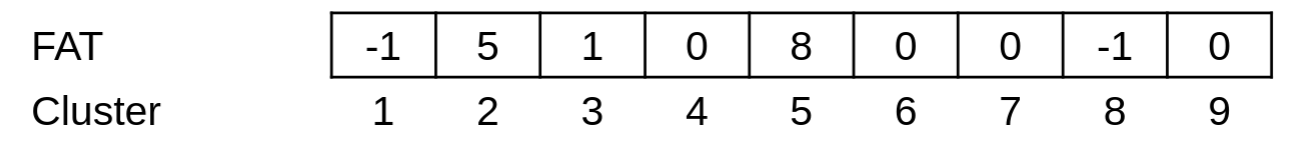
\includegraphics[width=0.99\linewidth]{clusters.png}
  \end{center}
\end{figure}
\begin{itemize}
    \item En el cluster 1 el valor correspondiente es -1: el archivo A arranca
          en el cluster 3, y almacena 512 bytes de los 680 que tiene el archivo.
          Como el cluster 3 tiene el valor 1, significa que debo ir al cluster 1
          y guardar el resto del archivo (168 bytes) allí. Como no hay más bytes
          para guardar, ponemos un -1 en el cluster 1 indicando el fin del archivo.
    \item El archivo B arranca en el cluster 2, observemos que el único valor posible
          al que puede apuntar el cluster 2 es al 5, porque el resto están libres
          o utilizados por el archivo A. Al cluster 8 tampoco puede apuntar porque
          ya lo está haciendo el cluster 5 y sería una inconsistencia. Por lo tanto,
          se almacenan los primeros 512 bytes en el cluster 2, los segundos 512 en el
          5, y el resto, va a parar al único cluster disponible que es el 8, que se 
          completa con el valor -1 porque ya no hay más bytes para almacenar.
\end{itemize}

\section*{Ejercicio 2}

\begin{figure}[h!]
  \begin{center}
    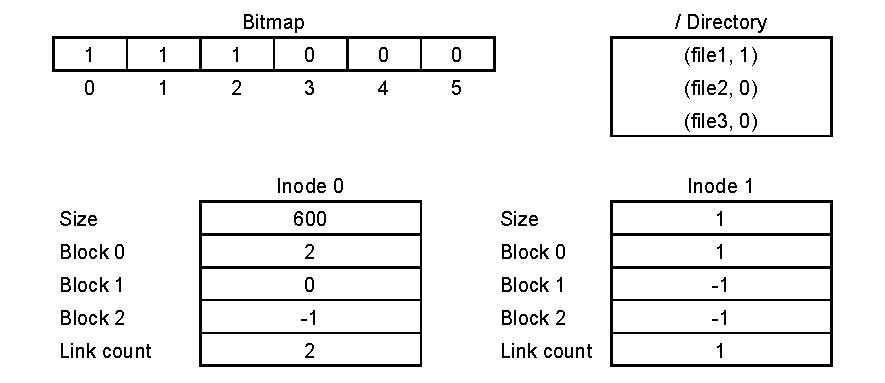
\includegraphics[width=0.99\linewidth]{unixfs.pdf}
  \end{center}
\end{figure}

\begin{itemize}
    \item El archivo del inodo 0 ocupa 600 bytes, por lo que además de almacenar
          512 bytes en el bloque 2 del disco, los 88 restantes se almacenarán
          en el bloque 0 (suponiendo que en el disco solo se encuentran los
          3 archivos listados en el directorio /).
    \item El archivo del inodo 1 ocupa un solo byte, por lo que alcanza con
          utilizar solo el bloque 1 del disco, los demás bloques del inodo
          estarán en -1.
    \item Los bits restantes del bitmap estarán apagados ya que no hay más archivos
          ocupando espacio que los dos mencionados anteriormente.
    \item Como en el inode 0 el link count es 2, podemos suponer que el file3
          apunta a este inodo, resultando también que el link count del inodo 1
          sea 1.
\end{itemize}

\section*{Ejercicio 3}

\subsection*{Apartado a)}

El inconveniente que puede surgir es que figuren como ocupados los clusters, 
pero en realidad no se están usando ya que el paso 4 no llegó a completarse, por
lo que no hay ninguna entrada que apunte a esta cadena de clusters. Esto podría
detectarse si ninguna entrada en el directorio apunta a alǵun nodo de esta cadena
(en especial al primero). Una vez detectado esto, se puede corregir
volviendo a marcar estos clusters como libres así pueden ser usados nuevamente. \\

Si este problema no se solucionara representaría un desperdicio de espacio, ya que
los clusters figuran como ocupados pero no están siendo utilzados por nadie.

\subsection*{Apartado b)}

El inconveniente que puede surgir en este caso es un poco más complejo, 
puede suceder que la entrada en el directorio esté apuntando a un cluster libre
o que esté apuntando a un cluster que está siendo utilizado por otro archivo.
Esto se puede detectar por ejemplo, siguiendo la cadena de clusters y viendo si
el tamaño no concuerda o viendo si este supuesto primer cluster de la cadena está
siendo apuntado por otro cluster, lo que significa que la entrada es inválida.
Teniendo en cuenta estos primeros casos, se puede solucionar fácilmente borrando
del directorio la entrada inválida. Luego también existe la posibilidad de que 
este espacio esté siendo ocupado por otro archivo que comienza en el mismo cluster
y necesitan ocupar la misma cantidad de clusters, este error es mucho más dificil
de corregir y se detectaría solamente al ir comparando todas las entradas
del directorio dos a dos. \\

Si este problema no es corregido, puede ocurrir que al intentar acceder a ese
archivo corrupto, se esté accediendo en realidad a información correspondiente
a otro archivo que haya ocupado los mismos clusters o a información basura
de un archivo borrado anteriormente en el mismo espacio.

\end{document}